\subsubsection{Langeweile} \label{langeweile-1}

\todo[inline]{Verantwortlich: Boris\\
- RfP}

Langeweile wird im Allgemeinen als eine Emotion wahrgenommen, die man erlebt, wenn man einen Zustand durchläuft, an dem man kein Interesse hat\cite{vodanovich_2003}. 
Dieses Gefühl charakterisiert Inaktivität, Unproduktivität und kann manchmal zu Melancholie oder Traurigkeit führen.
In dieser Studie wird das Erwachen der Langeweile durch eine grüne rotierende Scheibe mit einem schwarzen Strahl verursacht. \\

Für das erste Prototyp wird zwei Szenarios benutzt um die Langweile bei Probanden zu erwecken.
Als ersten wurde eine 5 minütigen Video über die "Latente Steuer im Jahres Abschluss" von der Tax Universität (https://www.youtube.com/watch?v=nhcG8zC7G2o) benutzt um diese Emotion auszulösen. 
Dabei ging es um eine kurze Einführungsvideo über Auswirkung von Latentesteuer in der Jahresbilanz.
Als zweites Szenario würde das ``Peg-Turning'' Spiel benutzt. 
Sein Prinzip besteht darin, alle 3 Sekunden eine grüne Scheibe durch ein Mausklick zu drehen. \\



\begin{figure}[H] \centering
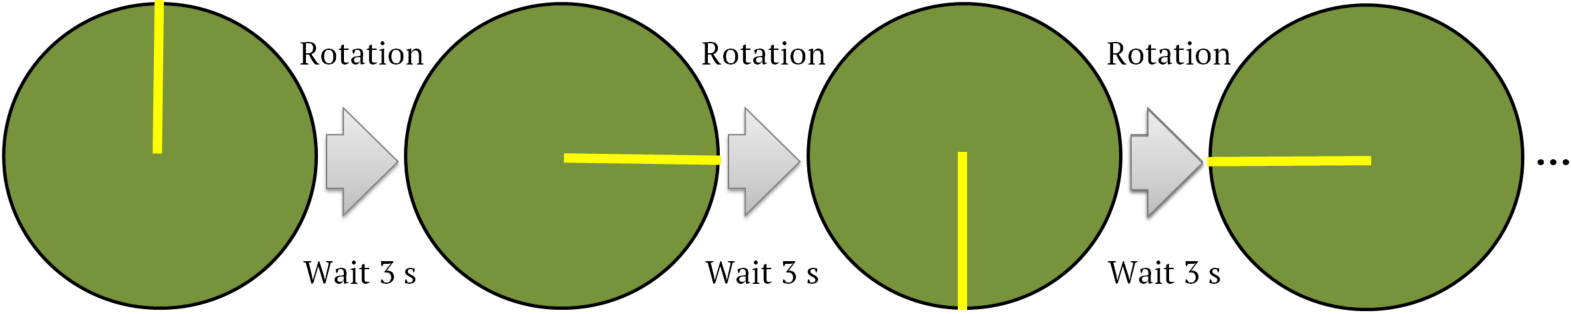
\includegraphics[width=\textwidth]{Images/boredom_game2.png} 
\vspace{-0.3cm} 
\caption{Bild des Langeweile-Szenarios.}
\label{fig-glueck} 
\end{figure}

